\documentclass[text04.tex]{subfiles}
\begin{document}
%538
\newpage
\subsection{ミニサッカーゲームで遊んでみよう}



文字とかんたんな\ruby{図形}{ず|けい}を使うだけでもゲームを作ることができます。実際にできあがっているプログラムを動かして試してみましょう。

スクリプトエディタの、ファイル→「開く」メニューから「kick.hsp」を読み込みましょう。

作業は、すべて「/home/ユーザー名/04」フォルダで行ないます。

見つからない場合は、まわりの友達か、近くの先生に聞いてみてください。



[F5]キーで実行すると、ミニサッカーゲームが動きます。



\begin{figure}[H]
    \begin{center}
      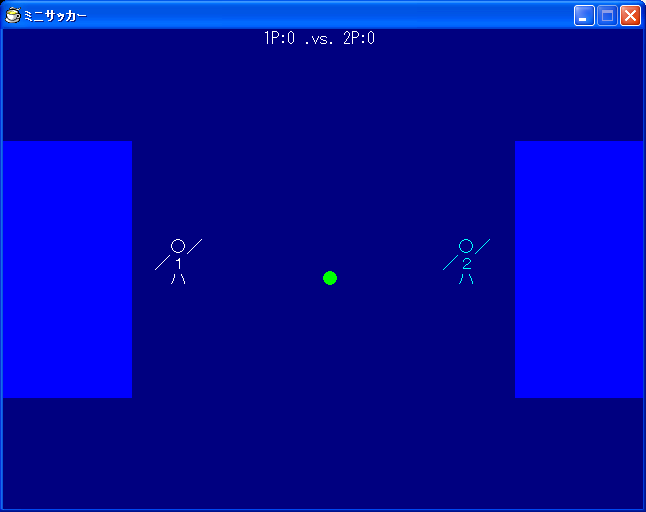
\includegraphics[keepaspectratio,width=9.075cm,height=7.197cm]{../../asset/image/s_kick.png}
      \caption{ミニサッカーゲームの画面}
    \end{center}
\end{figure}


このゲームは二人で\ruby{対戦}{たい|せん}します。

\ruby{隣}{となり}の席にいる人と、２人１組になって\ruby{一緒}{いっ|しょ}に遊んでみてください。

左側の「１」の人をキーボードの左側で\ruby{操作}{そう|さ}します。




\ \ \ \ [W]

[A] \ \ \ \ [D] \ \ \ \ [S] = ゴール前にもどる

\ \ \ \ [X]



右側の「２」の人をキーボードの右側で操作します。




\ \ \ \ [↑]

[←] \ \ \ [→] \ \ \ \ [Enter] = ゴール前にもどる

\ \ \ \ [↓]




それぞれのプレイヤーは足でボールを蹴って遠くに飛ばすことができます。

\ \ \ \ 「1」の人は右のゴールへ、

\ \ \ \ 「2」の人は左のゴールへボールを入れたら点が入ります。


\ \ \ \ ３点先に取った人の勝ちです。

\ \ \ \ 同じグループの友達と対戦してみましょう。



\begin{lstlisting}[caption=ミニサッカーゲームのプログラムの一部]
#include "hsp3dish.as"
world_x = 640; ウィンドウ全体のＸ座標
world_y = 480;ウィンドウ全体のＹ座標
bpx = 0 : bpy = 0       ; ボールの移動量
gsx = 128 : gsy = 256   ; ゴールのX,Yサイズ
gx1 = 0 : gy1 = 112     ; ゴール1のＸ座標Ｙ座標
gx2 = 512 : gy2 = 112   ; ゴール2のＸ座標Ｙ座標
kickx = 1.8             ; キックでボールが動く強さX
kicky = 2.0             ; キックでボールが動く強さY

randomize
*menu

screen 0, world_x, world_y

        title "ミニサッカー"
        repeat

        redraw 0
        font msgothic, 80, 1
        pos 80,140 : mes "ミニサッカー"
        font msgothic, 32, 0
        pos 170, 300 : mes "Enterキーでスタート"
        redraw 1

        await 30
        getkey a, 13 : if a : break

        loop

        cls 4
        score1 = 0
        score2 = 0

*main2
\end{lstlisting}


\newpage
\subsection{例題に挑戦しよう}

終わってしまった人は、以下の例題にも挑戦してみよう。


・ミニサッカーゲームの人を改造する

・ミニサッカーゲームのボールや色を変える

・ミニサッカーゲームの動きを改造する



例題の考え方がわからない時は、近くのTAか先生に聞いてください。

わからない所は、そのままにせず、必ず答えを見つけてから先に進みましょう。
\newpage
\subsection{\useOmetoiExample　ミニサッカーゲームの人を\ruby{改造}{かい|ぞう}する}

\exampleinduction

ミニサッカーゲーム(kick.hsp)のプログラムを改造してゲームの内容を変えてみましょう。

このゲームに\ruby{登場}{とう|じょう}する人は、実は文字の組み合わせで作られています。

\ruby{顔文字}{かお|も|じ}(\^{}\^{}) みたいですね。


\begin{lstlisting}[firstnumber=64,caption=ミニサッカーゲームのプログラムの一部]
;人1を表示するところ-------------------------------------------------------------------------

    color 255,255,255 ;白

    pos x1, y1 + 0 * 16 : mes "　○／"
    pos x1, y1 + 1 * 16 : mes "／１　"
    pos x1, y1 + 2 * 16 : mes "　ハ　"

;人2を表示するところ-------------------------------------------------------------------------

    color 0,255,255 ;水色

    pos x2, y2 + 0 * 16 : mes "　○／"
    pos x2, y2 + 1 * 16 : mes "／２　"
    pos x2, y2 + 2 * 16 : mes "　ハ　"

    redraw 1
;表示終わりウェイト--------------------------------------------------------------------------
\end{lstlisting}



プログラムから、mes命令で人を表示している部分を探して改造してみましょう。

mes命令は、

\deschspsyntax{mes “文字”}


のように必ず「”」の記号で文字を囲む必要があるので忘れないでください。

\exampleanswer


[F5]キーを押して改造した人がきちんと表示されるかどうか確認しましょう。

\ \ \ \ 人を改造することで、見た目が変わってあなただけのゲームに変わります。

改造ができたらTAや周りの友達にも見せてあげましょう。

\clearpage

\subsection*{[\ruby{重要}{じゅう|よう}]エラーが出て動かなくなった時は}

プログラムを改造していると、[F5]キーを押して実行しようとしても、エラーが\ruby{発生}{はっ|せい}して動かなくなったり、絵がおかしくなったりすることがあります。


\begin{figure}[H]
    \begin{center}
      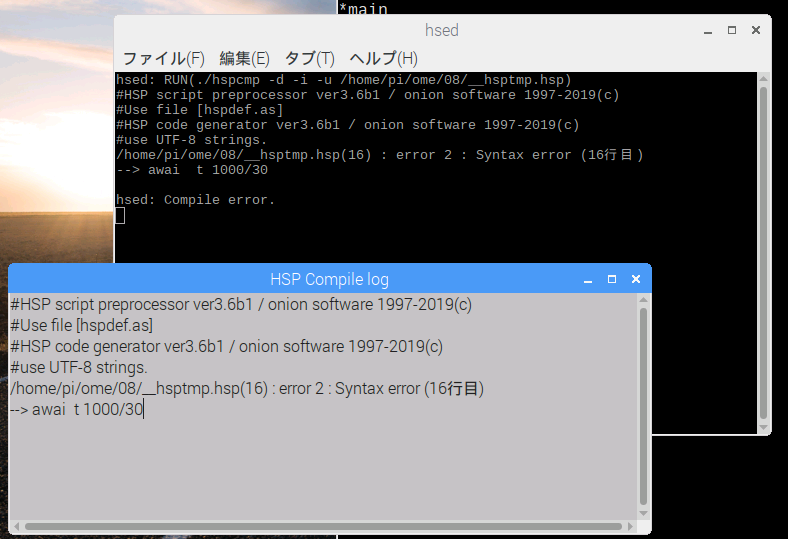
\includegraphics[keepaspectratio,width=11.324cm,height=7.756cm]{../../asset/image/s_hsperror.png}
      \caption{エラーの表示}
    \end{center}
\end{figure}

エラーが発生した時は、エラーの内容と「(xx行目)」というエラーの場所が示されます。

エディタの左下にカーソルがある行番号が表示されているので、エラーの場所を見直してください。

わからない時は、先生かTAに質問してみましょう。

どうしても動かなくなってしまった時には、元になっているファイルが保存されているので、

「/usr/local/share/ome/04」フォルダ内の元のファイル(kick.hsp)をもう一度コピーして使ってみてください。
%770
\newpage
\subsection{\useOmetoiExample　ミニサッカーゲームのボールや色を変える}

\exampleinduction

ミニサッカーゲーム(kick.hsp)のプログラムを改造してゲームの内容を変えてみましょう。

ゲームの中に出てくるサッカーボールもmes命令によって表示されています。


\begin{lstlisting}[firstnumber=48,caption=ミニサッカーゲームのプログラムの一部]
;全画面を消すところ-    -       -       -       -       -       -       -       -
    redraw 0

    color 0,0,128 : pos 0, 0: boxf ;画面クリア
    color 0,0,255
    boxf gx1,gy1,gx1+gsx,gy1+gsy
    boxf gx2,gy2,gx2+gsx,gy2+gsy

    color 255,255,255
    pos world_x / 2 - 60, 0 : mes "1P:" + score1 + " .vs. 2P:" + score2

;ボールを表示するところ----------------------------------------------------------------------

    color 0, 255, 0 ;グリーン
    pos bx, by : mes "●"

\end{lstlisting}


このボールも変えることができます。

プログラムの中から、ボールを出している部分を探して変更しましょう。



color命令は、色を決める命令だということを覚えていますか?

第2回で覚えたcolor命令の使い方を思い出しながら、ボールの色を変えてみましょう。

\begin{itembox}[c]{color命令の使い方}
    \deschspsyntax{color 赤の明るさ, 緑の明るさ, 青の明るさ}
    \begin{itemize}
        \item 色を変えるにはcolor命令を使います
        \item colorの後にスペースに続けて3つの数字を指定します
        \item 3つの数字は「,」で区切ること
        \item 0は暗い光、255は明るい光になります
    \end{itemize}
\end{itembox}

このゲームでは画像を一切使っていません。

背景のゴール、人、ボールも含めてすべてプログラムの中で決めています。

boxf命令は、好きな大きさの\ruby{四角形}{し|かく|けい}を画面に出すことのできる命令です。

この命令とcolorを組み合わせて背景となる色やゴールを出しています。



\ruby{実際}{じっ|さい}に色を書き\ruby{換}{か}えて、オリジナルのサッカーゲームを作ってみましょう。

タイトルの文字や、得点を表示する文字も変えることができます。




\exampleanswer


[F5]キーを押して改造した部分がきちんと表示されるかどうか確認しましょう。

\ \ \ \ プログラムを改造することで、見た目が変わってあなただけのゲームに変わります。

改造ができたらTAや周りの友達にも見せてあげましょう。
%861
\newpage
\subsection{\useOmetoiExample　ミニサッカーゲームの動きを改造する}

\exampleinduction

ミニサッカーゲーム(kick.hsp)のプログラムを改造してゲームの内容を変えてみましょう。

このプログラムでは、変数を使って人の動きや、ボールの動きを計算しています。

変数の代入と計算の方法を覚えていますか?



プログラムの最初に、変数に値を代入しています。

この値を変更することで、ゲームの動きが大きく変わります。


\begin{lstlisting}[firstnumber=3,caption=ミニサッカーゲームのプログラムの一部]
world_x = 640; ウィンドウ全体のＸ座標
world_y = 480;ウィンドウ全体のＹ座標
bpx = 0 : bpy = 0       ; ボールの移動量
gsx = 128 : gsy = 256   ; ゴールのX,Yサイズ
gx1 = 0 : gy1 = 112     ; ゴール1のＸ座標Ｙ座標
gx2 = 512 : gy2 = 112   ; ゴール2のＸ座標Ｙ座標
kickx = 1.8             ; キックでボールが動く強さX
kicky = 2.0             ; キックでボールが動く強さY
\end{lstlisting}


でたらめに書き直してもエラーになったり、処理が遅くなったりするので、あまり大きく変えないようにしましよう。

どの変数が、どのような働きをしているかをコメントとして書いてあります。


\deschspsyntax{変数 = 数字       ; コメント}

となっている時、「; コメント」の部分は、プログラムの実行には関係ないですがメモを残す意味で、文字が書かれています。「;」記号から後ろはコメントとして扱われるルールだということを覚えておきましょう。

Xは横方向の動きを表しています。Yは縦方向です。

数字を変えてどのように変わるか試してみましょう。


\exampleanswer



「kickx = 1.8」の数字を少しだけ大きくしてみましょう。

(大きくしすぎないようにしてください)

「kicky = 2.0」なども変えてみると、どうなるか確認してみましょう。



[F5]キーを押して改造したゲームがきちんと動くか確認しましょう。

改造ができたらTAや周りの友達にも見せてあげましょう。

\end{document}
